\documentclass{cubeamer}

\usepackage{graphicx}

\usepackage[sfdefault]{FiraSans}
\setsansfont[
  BoldFont={Fira Sans SemiBold},
  ItalicFont={Fira Sans Italic},
  BoldItalicFont={Fira Sans SemiBold Italic}
]{Fira Sans}

% math stuff
\usepackage{amsmath}                % to use DeclareMathOperator
\usepackage{amssymb}
\usepackage{mathrsfs}
\usepackage{mathtools}
\usepackage{xargs}                  % for more than one optional arguments when define new commands
\usepackage{physics}                % vectors
\usepackage{mdframed}               % frames for definition, theorem, etc.
\usepackage[ruled]{algorithm2e}     % for algorithms
\usepackage{ifthen}                % for \ifthenelse
\usepackage{upgreek}

% formatting some important single letters
\renewcommand{\epsilon}{\varepsilon}
\renewcommand{\phi}{\varphi}
\renewcommand{\upepsilon}{\upvarepsilon}
\renewcommand{\upphi}{\upvarphi}

% new operators
\DeclareMathOperator*{\argmin}{arg\,min}                % argmin
\DeclareMathOperator*{\argmax}{arg\,max}                % argmax
\DeclarePairedDelimiter\ceil{\lceil}{\rceil}            % ceiling function
\DeclarePairedDelimiter\floor{\lfloor}{\rfloor}         % floor function
\DeclarePairedDelimiter{\parens}{\lparen}{\rparen}      % parenthesis (use \parens* for automatically adjusting version)
\DeclarePairedDelimiter{\bracket}{[}{]}
\DeclarePairedDelimiter{\cbracket}{\{}{\}}
% \DeclarePairedDelimiter{\fourier}{\mathscr{F}\{}{\}}
% \DeclarePairedDelimiter{\invfourier}{\mathscr{F}^{-1}\{}{\}}

\newcommand{\fourier}[1]{\mathscr{F}\cbracket*{#1}}
\newcommand{\invfourier}[1]{\mathscr{F}^{-1}\cbracket*{#1}}
\newcommand {\dx}{\,dx}
\newcommand {\dy}{\,dy}
\newcommand {\dz}{\,dz}
\newcommand {\dt}{\,dt}
\newcommand {\du}{\,du}
\newcommand {\dtheta}{\,d\theta}
\newcommand {\domega}{\,d\omega}



\newcommand{\bigo}[1]{\ensuremath{\mathcal{O}\parens*{#1}}}
% new commands
\newcommand{\st}{such that }
\newcommand{\w}{where }
\newcommand{\del}{\nabla}
\newcommand{\larrow}{\leftarrow}
\newcommand{\rarrow}{\rightarrow}
\newcommand{\tbf}{\textbf}
\newcommand{\tit}{\textit}
\newcommand{\col}{\operatorname{col}}
\newcommand{\mat}[1]{\begin{matrix} #1 \end{matrix}}
% \newcommand{\vect}[1]{\boldsymbol{\mathbf{#1}}}
\newcommand{\vf}[1]{\boldsymbol{\mathbf{#1}}}
\newcommandx*{\seq}[2][1,2]{\ensuremath{#1, \ldots, #2}}
\newcommandx*{\ssum}[3][1,2,3]{\ensuremath{\sum_{#1 = #2}^{#3}}}
\newcommandx*{\sint}[2][1,2]{\ensuremath{\int_{#1}^{#2}}}
% \newcommandx*{\func}[4][1,2,3,4]{\ensuremath{#1^{\parens{#2}}_{#3}\parens{#4}}}
% \newcommandx*{\val}[3][1,2,3]{\ensuremath{#1^{\parens{#2}}_{#3}}}

% \newcommandx*{\func}[4][1=f,2=x,3,4, usedefault]{
%     \ifthenelse{\equal{#3}{}}{\ensuremath{#1_{#4}\parens{\vf{#2}}}}{\ensuremath{#1^{\parens{#3}}_{#4}\parens{\vf{#2}}}}
% }
\newcommandx*{\func}[3][1=f,2,3, usedefault]{
    \ifthenelse{\equal{#2}{}}{\ensuremath{#1_{#3}}}{\ensuremath{#1^{\parens{#2}}_{#3}}}
}
\newcommandx*{\val}[3][1,2,3, usedefault]{
    \ifthenelse{\equal{#2}{}}{\ensuremath{\vf{#1}_{#3}}}{\ensuremath{\vf{#1}^{\parens{#2}}_{#3}}}
}

\newcommandx*{\Expect}[1][1, usedefault]{\ensuremath{\mathbb{E}_{#1}}}  
\newcommandx*{\Real}[1][1, usedefault]{\ensuremath{\mathbb{R}^{#1}}}                % set of real number
\newcommandx*{\Int}[1][1, usedefault]{\ensuremath{\mathbb{Z}^{#1}}}                 % set of integer
\newcommandx*{\Natural}[1][1, usedefault]{\ensuremath{\mathbb{N}^{#1}}}             % set of natural number
\newcommandx*{\normal}[2][1=0, 2=1, usedefault=!]{\ensuremath{\mathcal{N}(#1,#2)}}  % Gaussian distribution

% define frame environment
% \newmdtheoremenv{definition}{Definition}
% \newmdtheoremenv{proposition}{Proposition}
% \newmdtheoremenv{corollary}{Corollary}
% \newmdtheoremenv{lemma}{Lemma}
% \newmdtheoremenv{theorem}{Theorem}
% \newmdtheoremenv{remark}{Remark}

% define keywords for algorithm
\SetKwInOut{Input}{Input}
\SetKwInOut{Output}{Output}
\SetKwInOut{Parameter}{Parameter}

% \begin{theorem}{text}{label}
% refer as \ref{tha:label}

% equation numbering
\numberwithin{equation}{section}

%%%%%%%%%%%%%%%%%%%%%%%%%%%
\usepackage{listings}
\usepackage{xcolor}

\definecolor{codegreen}{rgb}{0,0.6,0}
\definecolor{codegray}{rgb}{0.5,0.5,0.5}
\definecolor{codepurple}{rgb}{0.58,0,0.82}
\definecolor{backcolour}{rgb}{0.95,0.95,0.92}

\lstdefinestyle{mystyle}{
    backgroundcolor=\color{backcolour},   
    commentstyle=\color{codegreen},
    keywordstyle=\color{magenta},
    numberstyle=\tiny\color{codegray},
    stringstyle=\color{codepurple},
    basicstyle=\ttfamily\footnotesize,
    breakatwhitespace=false,         
    breaklines=true,                 
    captionpos=b,                    
    keepspaces=true,                 
    numbers=left,                    
    numbersep=5pt,                  
    showspaces=false,                
    showstringspaces=false,
    showtabs=false,                  
    tabsize=2
}

\lstset{style=mystyle}

\title{Fast Underwater Image Enhancement for \\ Improved Visual Perception}
\author{Chinchuthakun Worameth}
\date{January 17, 2022}
\institute{Yamashita Laboratory \\ 
Department of Transdisciplinary Science and Engineering \\
School of Environment and Society \\
Tokyo Institute of Technology}

\begin{document}

\maketitle

% \cutoc

\section{Background}
\begin{frame}{Challenges of underwater imaging}
    \begin{itemize}
        \item Light propagation under water is different than in the atmosphere
        \begin{itemize}
            \item Basically \tbf{a different set of non-linear transformations} from real-world scenes to image (color) coordinate system
            \item For example, underwater images usually have \keyword{higher green or blue hues} because red wavelengths are absorbed in deep water region
        \end{itemize}
    \end{itemize}
    \begin{figure}
        \centering
        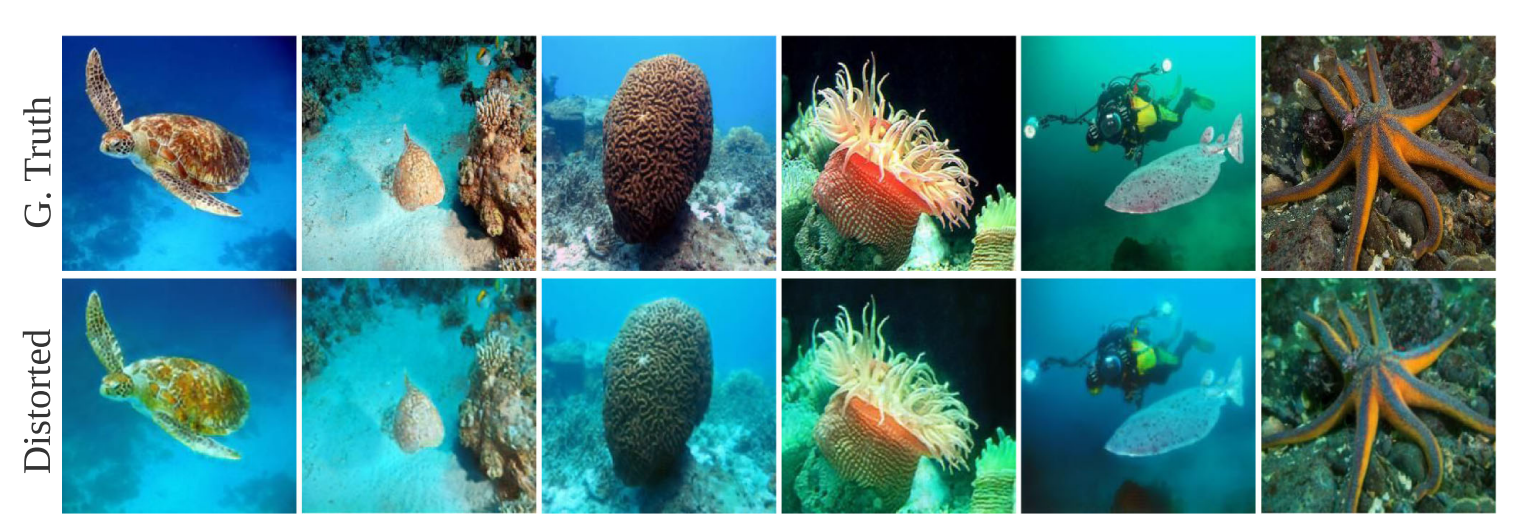
\includegraphics[width=.7\textwidth]{figures/paired-example.PNG}
        \caption{Paired instances from EUVP dataset \cite{funie-gan}}
    \end{figure}
\end{frame}

\begin{frame}{Challenges of underwater imaging (2)}
    \begin{itemize}
        \item We can perform \keyword{dehazing} and \keyword{color correction} using \keyword{physical models} with additional parameters, e.g. depth or optical water-quality measures
        \begin{itemize}
            \item Not always available in robotic applications
            \item \tbf{Multimodal models are computational expensive for real-time deployment}
        \end{itemize}
        \item Several models based on \keyword{CNN} and \keyword{GAN} are proposed
        \begin{itemize}
            \item Unfortunately, We could not achieve a good performance with deep learning
            \item \tbf{Underwater data are expensive and difficult to acquire!}
        \end{itemize}
    \end{itemize}
\end{frame}

\begin{frame}{Research overview}
    \begin{itemize}
        \item Published a \keyword{EUVP dataset (Enhancement of Underwater Visual Perception)}
        \begin{itemize}
            \item 12K paired and 8K unpaired underwater of poor and good quality
        \end{itemize}
        \item Presented a deep learning model for fast underwater image  enhancement
        \begin{itemize}
            \item Framed the problem as \keyword{image-to-image translation}
            \item Proposed a \keyword{conditional GAN architecture} to solve it
            \item Evaluated on the proposed dataset
        \end{itemize}
    \end{itemize}
\end{frame}

\begin{frame}{Background: Image-to-image translation}
    \begin{itemize}
        \item Transform \keyword{style} of images in one domain to another domain
        \item Some famous examples \textemdash ~ \keyword{Pix2Pix} \cite{pix2pix} and \keyword{CycleGan} \cite{cyclegan}
    \end{itemize}
    \begin{columns}
        \begin{column}{0.4\textwidth}
            \begin{figure}
                \centering
                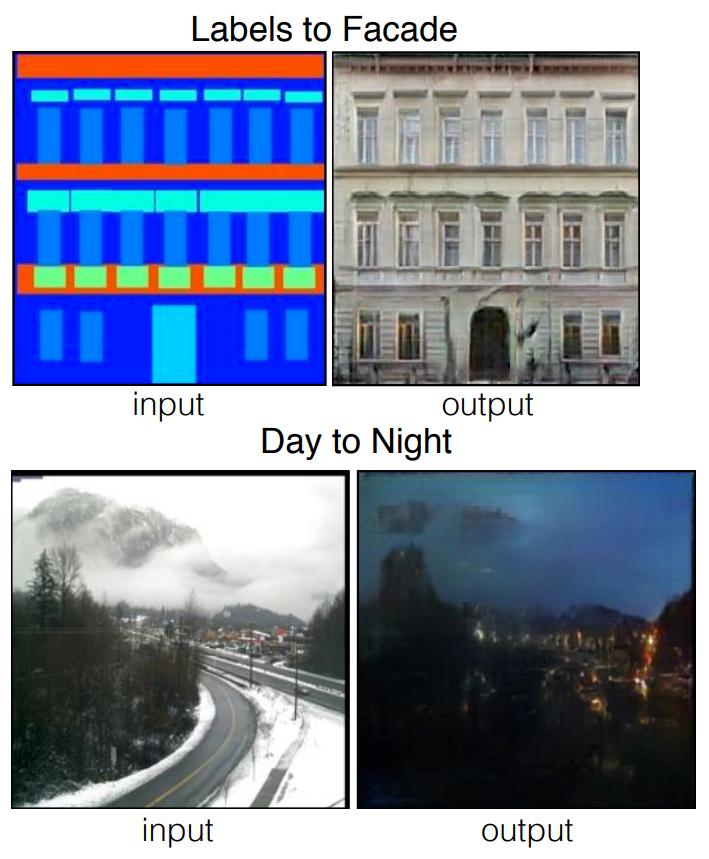
\includegraphics[width=0.7\columnwidth]{figures/pix2pix-example.PNG}
                \caption{Examples from Pix2Pix \cite{pix2pix}}
            \end{figure}
        \end{column}
        \begin{column}{0.5\textwidth}
            \begin{figure}
                \centering
                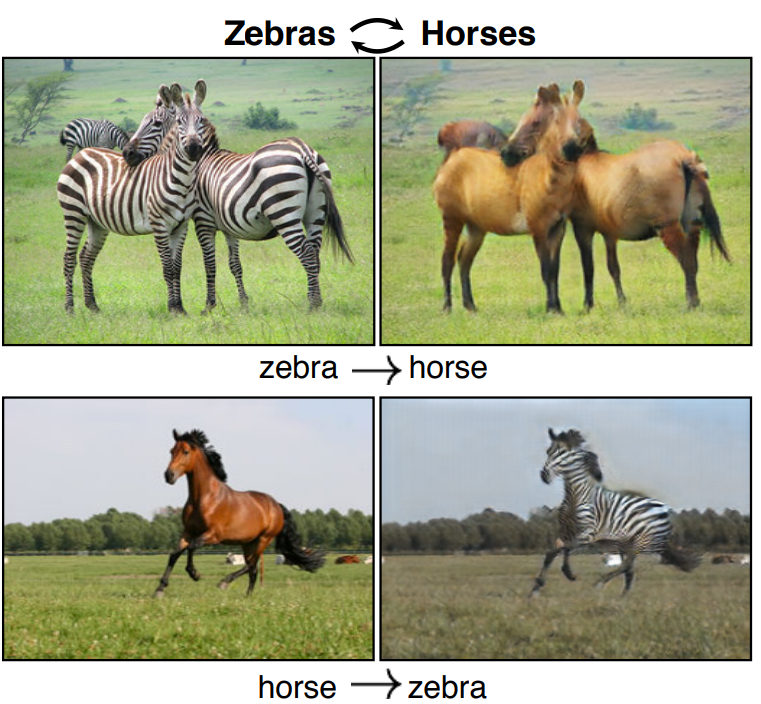
\includegraphics[width=0.7\columnwidth]{figures/cyclegan-example.PNG}
                \caption{Examples from CycleGAN \cite{cyclegan}}
            \end{figure}
        \end{column}
    \end{columns}
\end{frame}

\begin{frame}{Background: Recap of GAN}
    \begin{itemize}
        \item A two-player min-max game between \keyword{generator} and \keyword{discriminator}
        \item \keyword{Conditional GANs} impose constrains such that generators produce samples belonged to a specified class
    \end{itemize}
    \vspace{-0.5cm}
    \begin{figure}
        \centering
        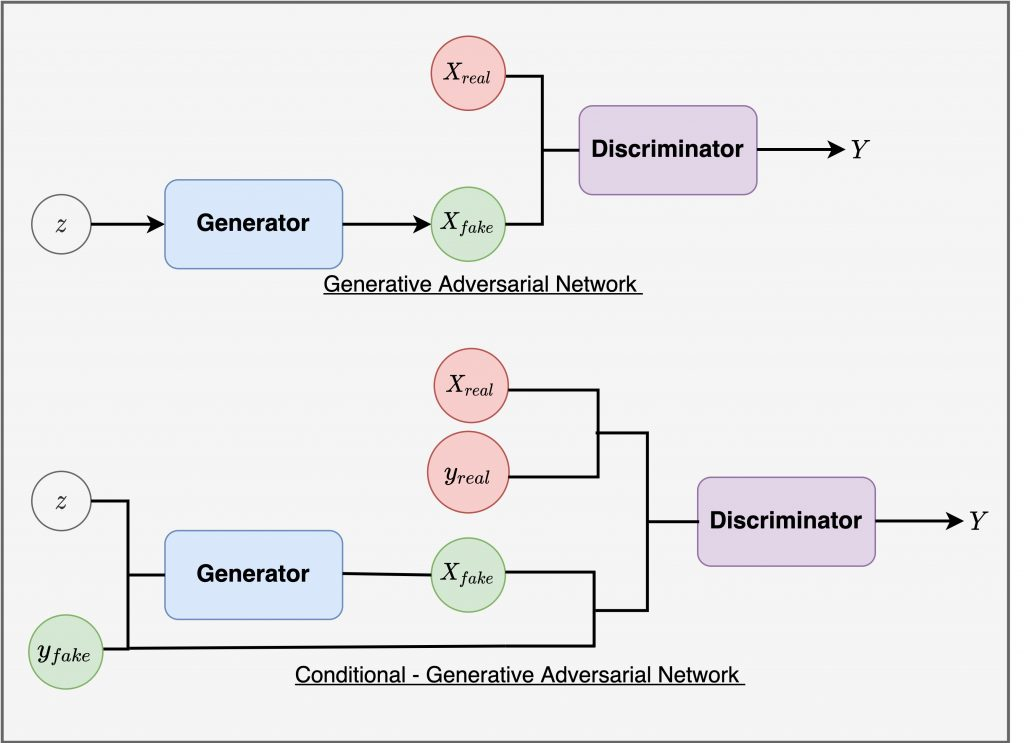
\includegraphics[width=.45\textwidth]{figures/gan-architecture.jpeg}
    \end{figure}
    \footnotetext[1]{\tiny Image available from \url{https://learnopencv.com/conditional-gan-cgan-in-pytorch-and-tensorflow/}}
\end{frame}

\begin{frame}{Background: Pix2Pix in a nutshell}
    \begin{itemize}
        \item Generator follows \keyword{U-Net architecture}
        \item Discriminator uses \keyword{PatchGAN}, predicting if patches of images are real or fake
    \end{itemize}
    \begin{figure}
        \centering
        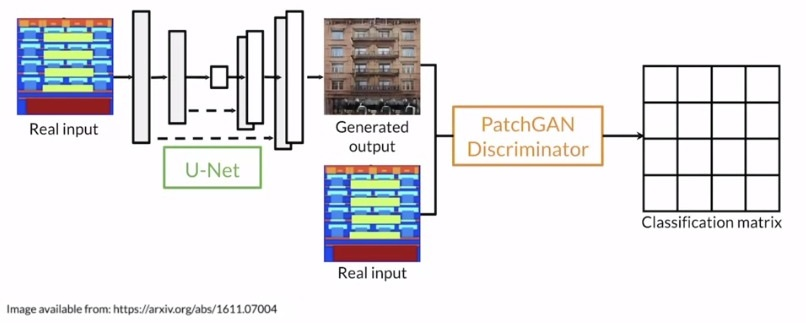
\includegraphics[width=.8\textwidth]{figures/pix2pix-architecture.jpg}
    \end{figure}
    \footnotetext[1]{\tiny Image available from \url{https://www.haikutechcenter.com/2020/10/pix2pix-gan-architecture-for-image-to.html}}
\end{frame}

\begin{frame}{Background: CycleGAN in a nutshell}
    \begin{itemize}
        \item Although Pix2Pix requires paired training data, we can solve this problem with \keyword{cycle-consistency loss}
    \end{itemize}
    \begin{figure}
        \centering
        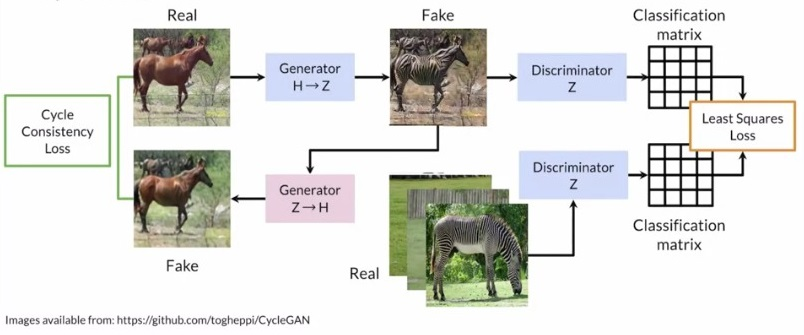
\includegraphics[width=.8\textwidth]{figures/cyclegan-architecture.jpg}
    \end{figure}
    \footnotetext[1]{\tiny Image available from \url{https://www.haikutechcenter.com/2020/11/cyclegan-gan-architecture-for-learning.html}}
\end{frame}

\begin{frame}{Methodology: Network Architecture}
    \begin{itemize}
        \item Following previous works, generator and discriminator are \tbf{mini U-Net} and \tbf{PatchGAN}, respectively.
    \end{itemize}
    \begin{figure}
        \centering
        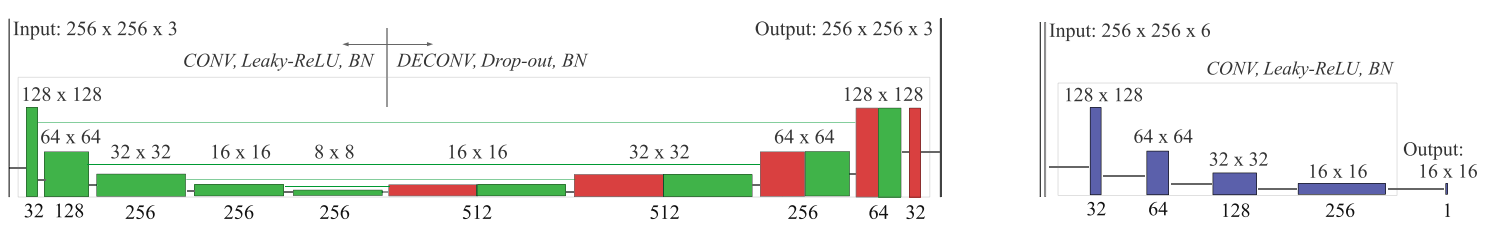
\includegraphics[width=1.0\textwidth]{figures/funie-architecture.PNG}
        \caption{Architecture of FUnIE-GAN \cite{funie-gan}}
    \end{figure}
\end{frame}

\begin{frame}{Methodology: Loss Function}
    \begin{itemize}
        \item \tbf{Paired image translation}
        
        Let $X, Y$ be the source and target domain. Consider an input $Z$ with a generator $G$ and discriminator $D$:
        \begin{itemize}
            \item \keyword{Adversarial Loss}
            $$
            L_{cGAN}(G,D) = \Expect[X,Y]\bracket*{\log D(Y)} + \Expect[X,Y]\bracket*{\log \parens*{1 - D(X, G(X,Z))}}
            $$
            \item \keyword{Global Similarity}
            $$
            L_{1}(G) = \Expect[X,Y,Z]\bracket*{\norm{Y - G(X,Z)}_1}
            $$
            \item \keyword{Image content}
            $$
            L_{con}(G) = \Expect[X,Y,Z]\bracket*{\norm{\Phi(Y) - \Phi(G(X,Z))}_2}
            $$
            where $\Phi$ denotes the image content function, i.e. the high-level features extracted by a certain layer of a pre-trained \keyword{VGG-19 architecture}
        \end{itemize}
    \end{itemize}
\end{frame}

\begin{frame}{Methodology: Loss Function (2)}
    \begin{itemize}
        \item \tbf{Paired image translation (con't)}
        $$
        G^* = \argmin_{G} \max_{D} L_{cGAN}(G,D) + \lambda_1 L_{1}(G) + \lambda_c L_{con}(G)
        $$
        \item \tbf{Unpaired image translation}
        \begin{itemize}
            \item Since we do not have access to the ground-truth image, we only use adversarial loss and cycle-consistency loss
            \item Let $G_F: \{X,Z\} \rarrow Y$ and $G_R: \{Y,Z\} \rarrow X$:
            $$
            G_F^*, G_R^* = \argmin_{G_F, G_R} \max_{D_Y, D_X} L_{cGAN}(G_F,D_Y) + L_{cGAN}(G_R,D_X) + \lambda_{cyc} L_{cyc} (G_F, G_R)
            $$
            where
            $$
            L_{cyc} (G_F, G_R) = \Expect[X,Y,Z]\bracket*{\norm{X - G_R(G_F(X,Z))}_1} + \Expect[X,Y,Z]\bracket*{\norm{Y - G_F(G_R(X,Z))}_1}
            $$
        \end{itemize}
    \end{itemize}
\end{frame}

\begin{frame}{Experiments: Qualitative Analysis}
    \begin{columns}
        \begin{column}{0.45\textwidth}
            \begin{figure}
                \centering
                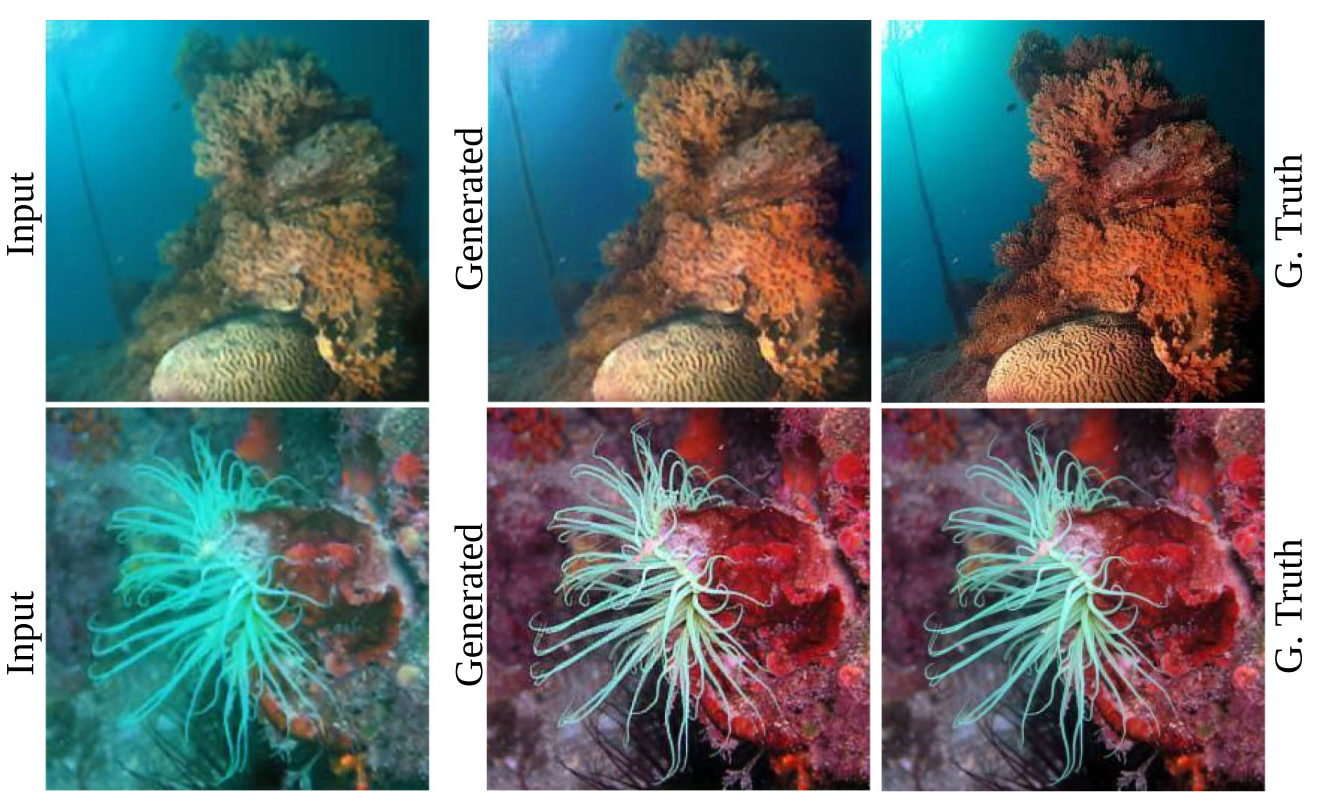
\includegraphics[width=0.8\columnwidth]{figures/result-1.PNG}
            \end{figure}
        \end{column}
        \begin{column}{0.45\textwidth}
            \begin{figure}
                \centering
                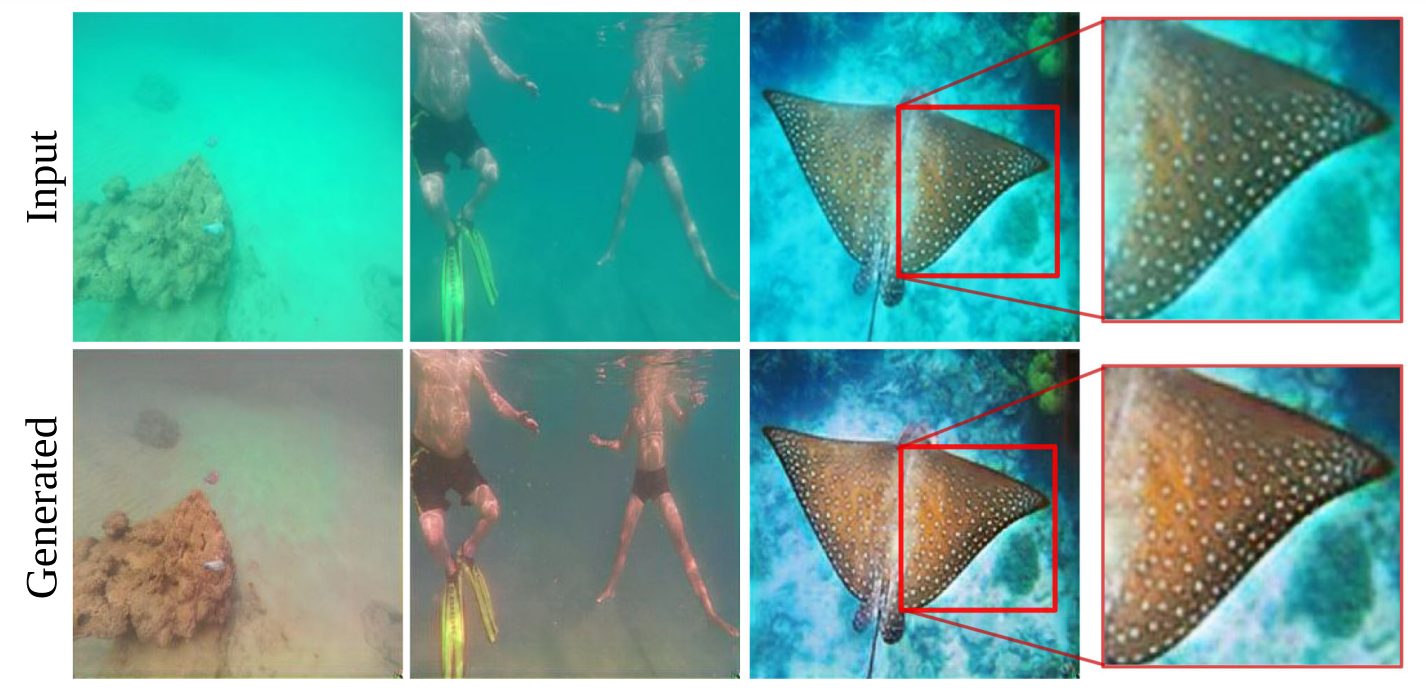
\includegraphics[width=1.\columnwidth]{figures/result-2.PNG}
            \end{figure}
        \end{column}
    \end{columns}
    \begin{figure}
        \centering
        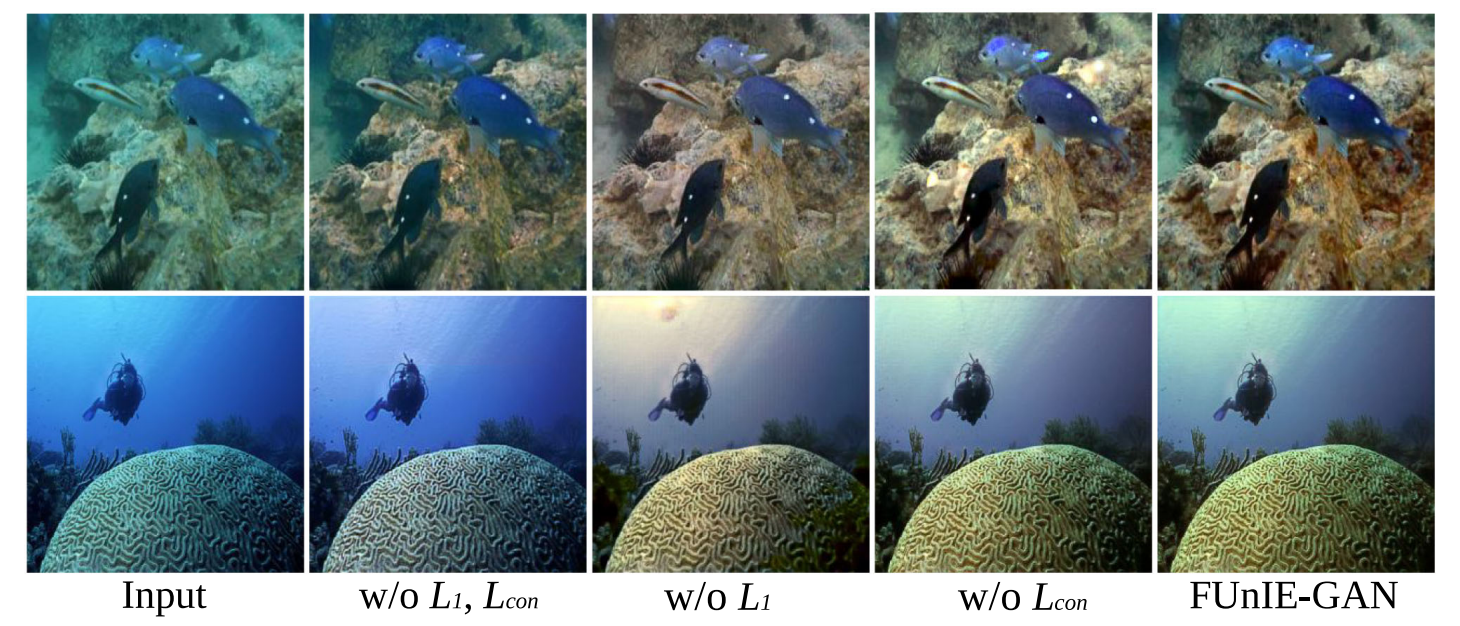
\includegraphics[width=0.5\columnwidth]{figures/result-3.PNG}
    \end{figure}
\end{frame}

\begin{frame}{Experiments: Quantitative Analysis}
    \begin{itemize}
        \item Three metrics are considered:
        \begin{itemize}
            \item \keyword{Peak Signal-to-Noise Ratio (PSNR)}: measure reconstruction quality
            $$
            PSNR(\val[x],\val[y]) = 10 \log_{10} \parens*{255^2 / MSE(\val[x],\val[y])}
            $$
            \item \keyword{Structural Similarity (SSIM)}: measure luminance, constrast, and structure
            $$
            SSIM(\val[x], \val[y]) = \parens*{\frac{2 \val[\mu][][{\val[x]}] \val[\mu][][{\val[y]}] + c_1}{\val[\mu][][{\val[x]}]^2 + \val[\mu][][{\val[y]}]^2 + c_1}} \parens*{\frac{2 \val[\sigma][][{\val[xy]}]+ c_2}{\val[\sigma][][{\val[x]}]^2 + \val[\sigma][][{\val[y]}]^2 + c_2}}
            $$
            \item \keyword{Underwater Image Quality Measure (UIQM)} \cite{uiqm}
            \begin{itemize}
                \item Quantifies underwater image colorfulness, sharpness, and contrast according to human visual perceptions.
            \end{itemize}
        \end{itemize}
    \end{itemize}
\end{frame}

\begin{frame}{Experiments: Qualitative Analysis and User Study}
    \begin{itemize}
        \item \tbf{Comparison with other state-of-the-arts}
        \begin{columns}
            \begin{column}{0.45\textwidth}
                \begin{figure}
                    \centering
                    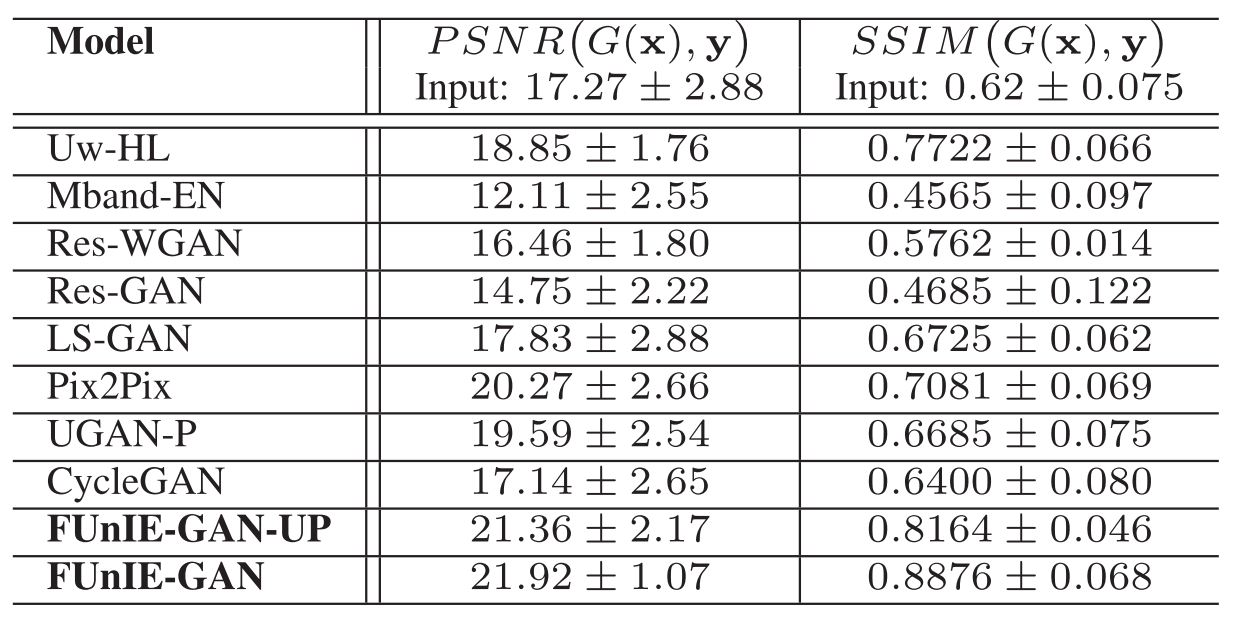
\includegraphics[width=1.0\columnwidth]{figures/result-4.PNG}
                \end{figure}
            \end{column}
            \begin{column}{0.45\textwidth}
                \begin{figure}
                    \centering
                    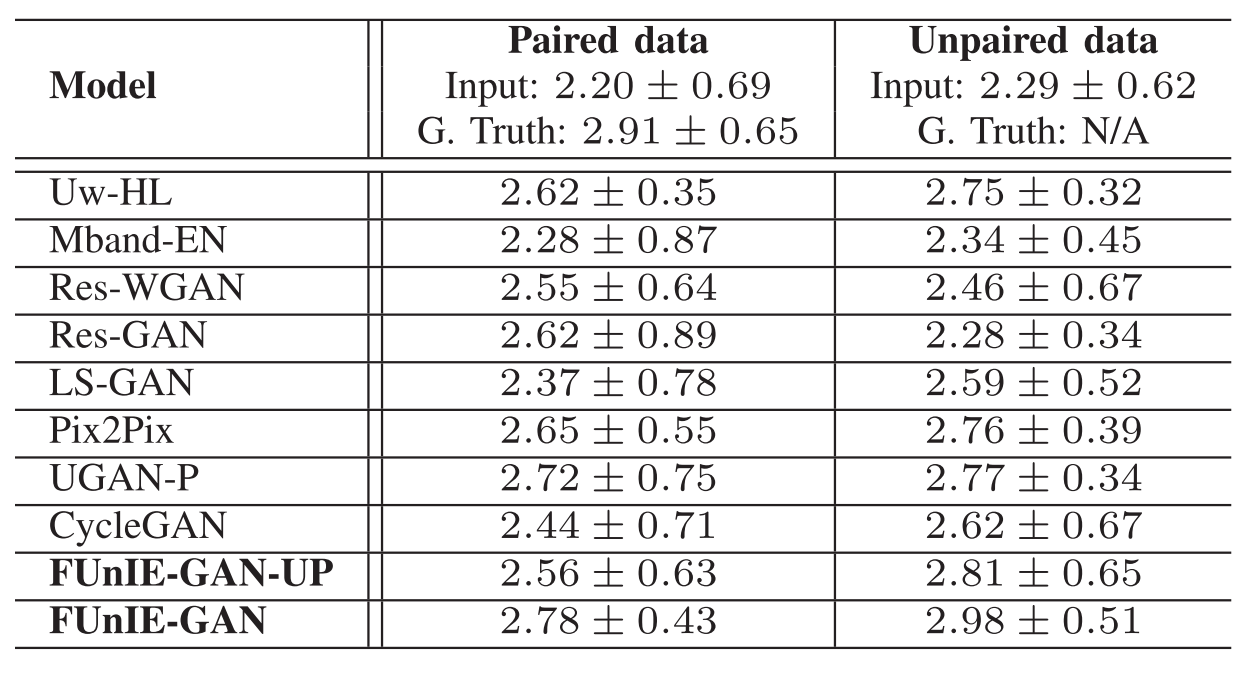
\includegraphics[width=1.\columnwidth]{figures/result-5.PNG}
                \end{figure}
            \end{column}
        \end{columns}
        \item \tbf{Human's preference on generated images}
        \begin{figure}
            \centering
            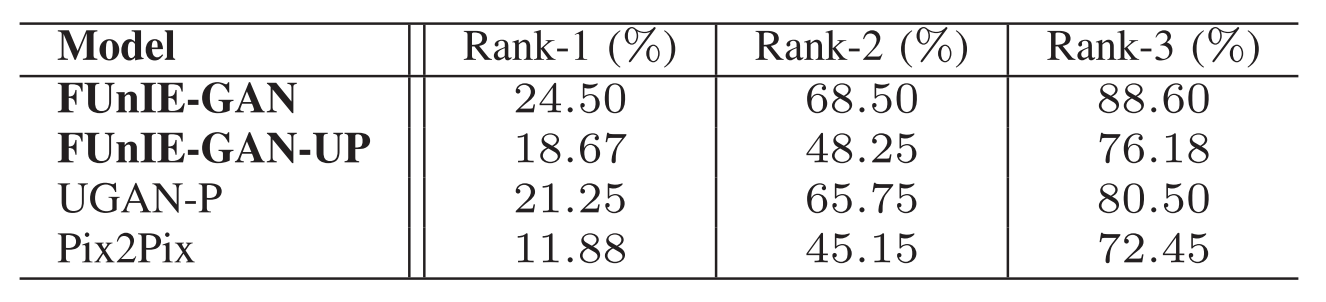
\includegraphics[width=0.5\columnwidth]{figures/result-6.PNG}
    \end{figure}
    \end{itemize}
\end{frame}

\begin{frame}{Experiments: Implication}
    \begin{columns}
            \begin{column}{0.3\textwidth}
                \begin{itemize}
                    \item Improve performance in downstream tasks
                \end{itemize}
            \end{column}
            \begin{column}{0.6\textwidth}
                \begin{figure}
                    \centering
                    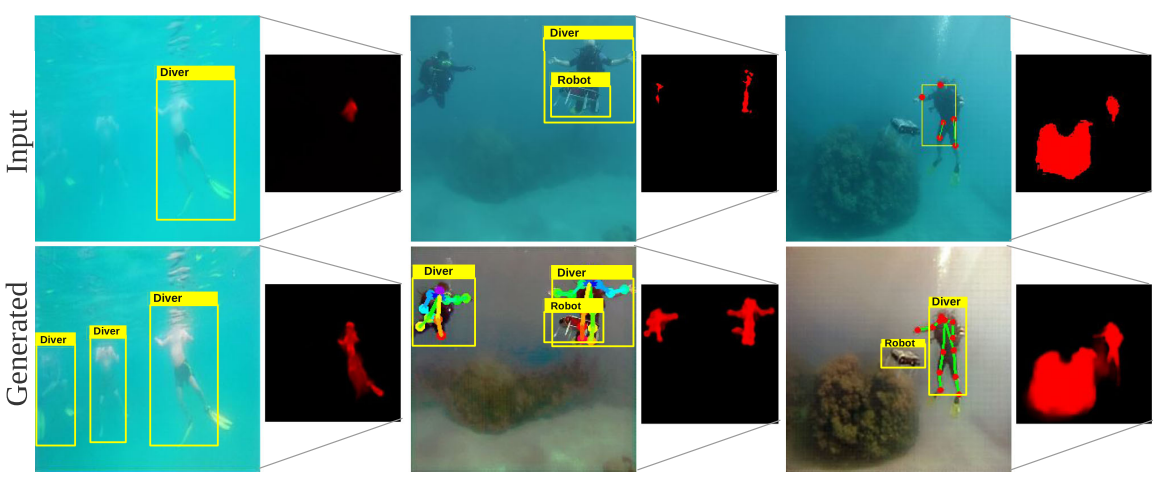
\includegraphics[width=1.0\columnwidth]{figures/result-7.PNG}
                \end{figure}
                \vspace{-0.5cm}
                \begin{figure}
                    \centering
                    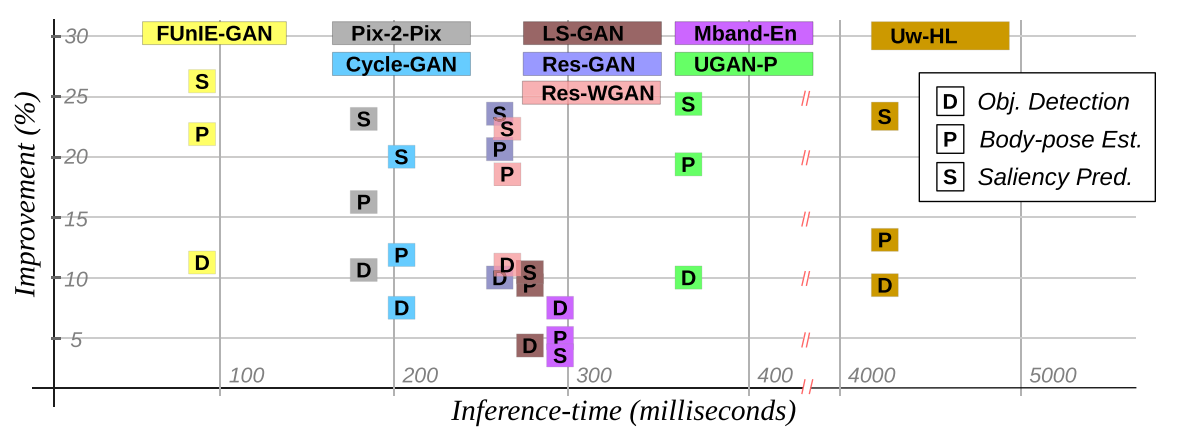
\includegraphics[width=1.0\columnwidth]{figures/result-8.PNG}
                \end{figure}
            \end{column}
    \end{columns}
\end{frame}

\begin{frame}{Limitations}
    \begin{itemize}
        \item Not very effective in severely degraded and texture-less images
        \item Require careful hyperparameter tuning in unpaired image-to-image translation; otherwise, the discriminator will become too good too early
    \end{itemize}
    \vspace{-0.5cm}
    \begin{figure}
        \centering
        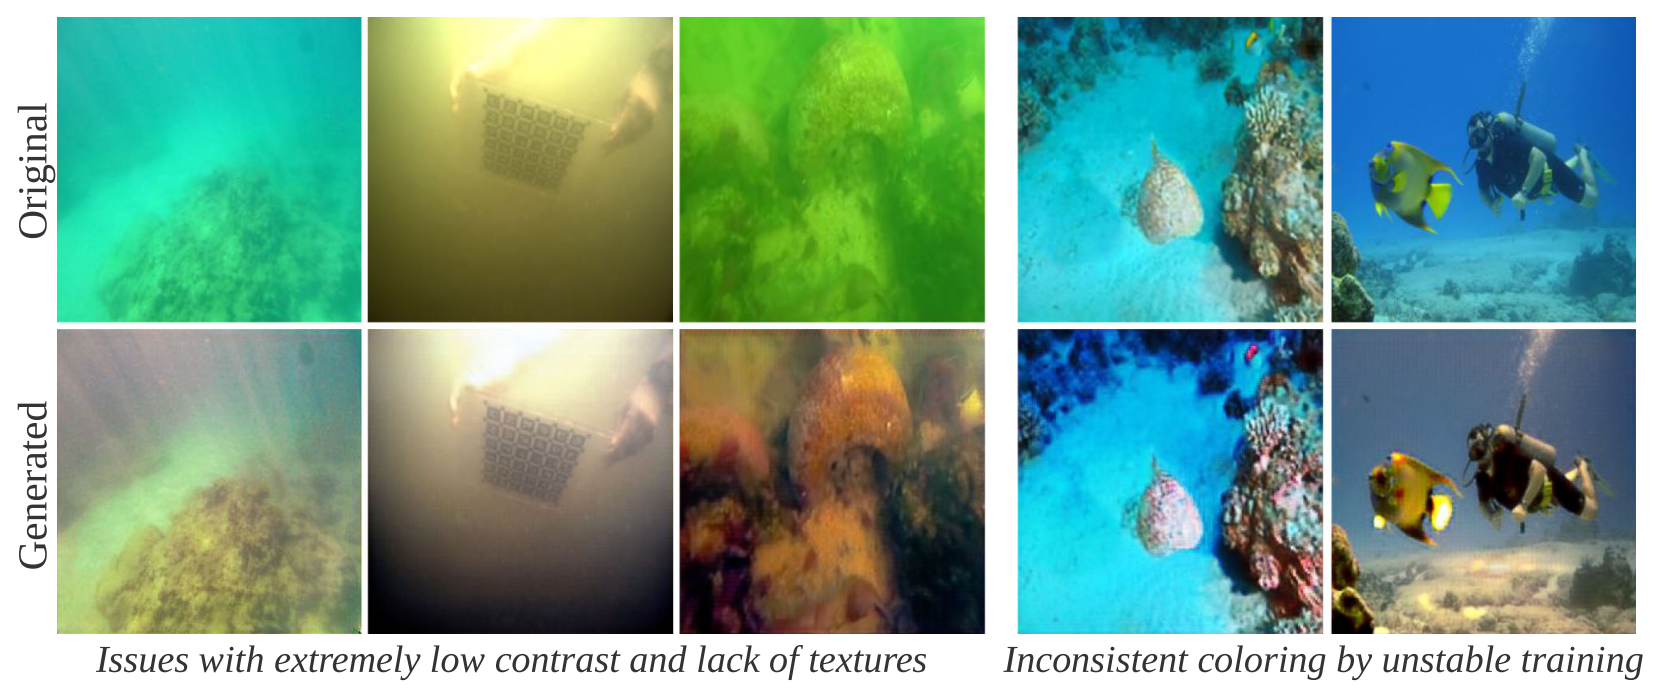
\includegraphics[width=0.8\textwidth]{figures/result-9.PNG}
    \end{figure}
\end{frame}

\setbeamertemplate{bibliography item}{\insertbiblabel}
\setbeamerfont{bibliography item}{size=\scriptsize}
\setbeamerfont{bibliography entry author}{size=\scriptsize}
\setbeamerfont{bibliography entry title}{size=\scriptsize}
\setbeamerfont{bibliography entry location}{size=\scriptsize}
\setbeamerfont{bibliography entry note}{size=\scriptsize}

\begin{frame}[allowframebreaks, noframenumbering]{References}
    \bibliographystyle{IEEEtran}
    \bibliography{references}
\end{frame}

\end{document}
